% DOCX body[12]
\begin{figure*}[pos=t]
\centering
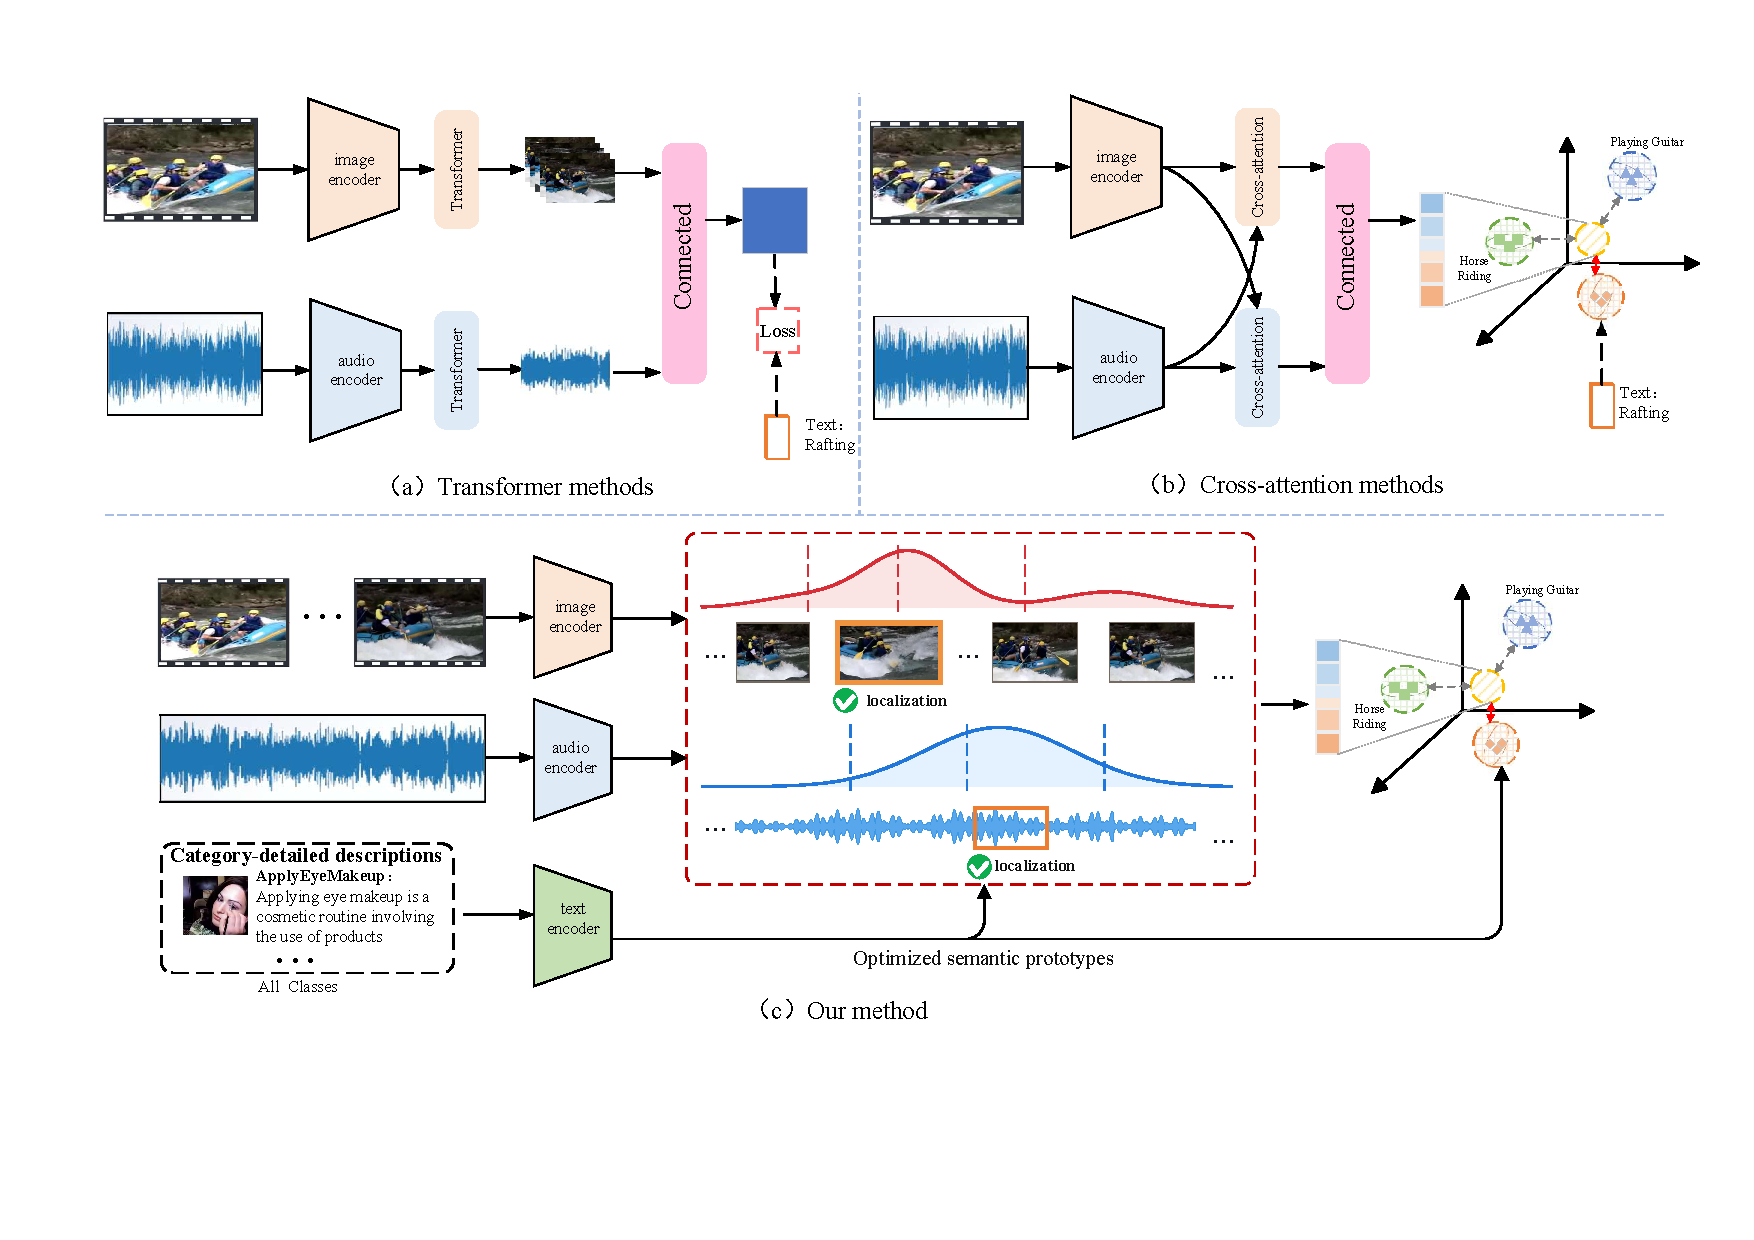
\includegraphics[pagebox=mediabox,width=\textwidth,trim={43bp 99bp 20bp 29bp},clip]{figures/Introduction.pdf}
\caption{Comparison of the proposed framework with existing AVGZSL methods. Transformer-based methods (a) emphasize intra-modal temporal modeling, whereas cross-attention-based methods (b) emphasize inter-modal interaction. Both follow the \textquotedblleft{}encode first, match later\textquotedblright{} paradigm without direct class-semantic guidance for temporal evidence selection. In contrast, our method (c) uses optimized class embeddings to guide independent Gaussian temporal aggregation for visual and audio sequences, adaptively localizes and aggregates class-relevant segments, and aligns the fused audio-visual representation with the class embeddings.}
\label{fig:comparison}
\end{figure*}
